% !TeX root = main.tex
\changecolours{ScoutRed}
\section[Estágios Avançados e Otimização]{Estágios Avançados, Otimização e Desempenho}

% ------------------------------------------------------------------------------
\begin{frame}[fragile]{O Estágio \texttt{\$facet}: Dashboards Multi-Perspectiva}
  \vspace{0.1cm}
  \begin{columns}[t,onlytextwidth]
    \begin{column}{0.46\textwidth}
      \alert{Processamento Paralelo em Passo Único}\par
      \footnotesize
      \begin{itemize}
        \item Executa múltiplos sub-pipelines independentes em paralelo sobre a mesma massa de dados.
        \item Permite alimentar múltiplos componentes de um painel (\textit{dashboard}) em uma única requisição.
        \item \textbf{Redução de Latência:} Elimina múltiplas idas e vindas de rede (\textit{Round-Trip Time}) com o servidor.
        \item Todos os sub-pipelines compartilham o mesmo estágio \lstinline[language=mongosh, basicstyle=\footnotesize\ttfamily]|$match| inicial.
      \end{itemize}
    \end{column}
    \begin{column}{0.52\textwidth}
      \alert{Sintaxe de Dashboard no MongoSH}\par
      \vspace{0.05cm}
      \begin{lstlisting}[language=mongosh, basicstyle=\scriptsize\ttfamily]
db.pedidos.aggregate([
  { $match: { status: "entregue" } },
  { $facet: {
      "kpis_gerais": [
        { $group: {
            _id: null,
            faturamento: { $sum: "$valor_total" },
            pedidos: { $sum: 1 }
        } }
      ],
      "por_canal": [
        { $group: { _id: "$canal", total: { $sum: "$valor_total" } } },
        { $sort: { total: -1 } }
      ]
  } }
])
      \end{lstlisting}
    \end{column}
  \end{columns}
\end{frame}

% ------------------------------------------------------------------------------
\begin{frame}[fragile]{Otimização do Pipeline e Gestão de Memória RAM}
  \vspace{0.1cm}
  \begin{columns}[t,onlytextwidth]
    \begin{column}{0.48\textwidth}
      \alert{O Teto Estrito de 100 MB por Estágio}\par
      \footnotesize
      \begin{itemize}
        \item Cada estágio do pipeline opera com limite máximo de \textbf{100 MB de RAM}.
        \item Operações de \lstinline[language=mongosh, basicstyle=\footnotesize\ttfamily]|$group| ou \lstinline[language=mongosh, basicstyle=\footnotesize\ttfamily]|$sort| sem índice que estourem o limite abortam com o erro:
          \par\vspace{0.1cm}
          \centering
          \lstinline[language=mongosh, basicstyle=\fontsize{7.2pt}{6pt}\ttfamily]|QueryExceededMemoryLimitNoDiskUseAllowed|
          \par\vspace{0.1cm}
          \raggedright
        \item \textbf{Cargas em Lote (\textit{Batch}):} Permita a escrita temporária em disco adicionando a opção:
          \par\vspace{0.1cm}
          \centering
          \lstinline[language=mongosh, basicstyle=\footnotesize\ttfamily]|{ allowDiskUse: true }|
      \end{itemize}
    \end{column}
    \begin{column}{0.48\textwidth}
      \alert{Otimizações Automáticas da Engine}\par
      \footnotesize
      \begin{itemize}
        \item \textbf{Otimização de Sequência:} O motor reordena os estágios \lstinline[language=mongosh, basicstyle=\footnotesize\ttfamily]|$match| para o início automaticamente.
        \item \textbf{Coalescência de \lstinline[language=mongosh, basicstyle=\footnotesize\ttfamily]|$match| e \lstinline[language=mongosh, basicstyle=\footnotesize\ttfamily]|$sort|:} Combina filtros e ordenações para navegar diretamente nas folhas da árvore B-Tree (Regra ESR).
        \item \textbf{Early Projection:} Descarta atributos não utilizados nas etapas seguintes para diminuir a pegada de memória.
      \end{itemize}
    \end{column}
  \end{columns}
\end{frame}

% ------------------------------------------------------------------------------
\begin{frame}[fragile]{Validação Empírica: Benchmark de Otimização}
  \vspace{0.1cm}
  \begin{columns}[t,onlytextwidth]
    \begin{column}{0.48\textwidth}
      \alert{Análise Comparativa dos 3 Cenários}\par
      \footnotesize
      \begin{itemize}
        \item \textbf{Cenário 1 (Não Otimizado):} O estágio \lstinline[language=mongosh, basicstyle=\footnotesize\ttfamily]|$unwind| expande 10.000 pedidos em mais de 25.000 documentos na RAM antes de filtrar. \textit{Latência: \textbf{142.6 ms}} (gargalo de memória).
        \item \textbf{Cenário 2 (Match Precoce):} Filtragem seletiva no estágio 1 descarta documentos cancelados antes da expansão. \textit{Latência: \textbf{52.8 ms}} ($2.7\times$ mais rápido).
        \item \textbf{Cenário 3 (Pipeline ESR Otimizado):} Filtro apoiado em índice B-Tree composto com projeção estrita. \textit{Latência: \textbf{14.1 ms}} ($>10\times$ mais veloz!).
      \end{itemize}
    \end{column}
    \begin{column}{0.50\textwidth}
      \alert{Medição Empírica (Tempo e RAM)}\par
      \vspace{0.05cm}
      \centering
      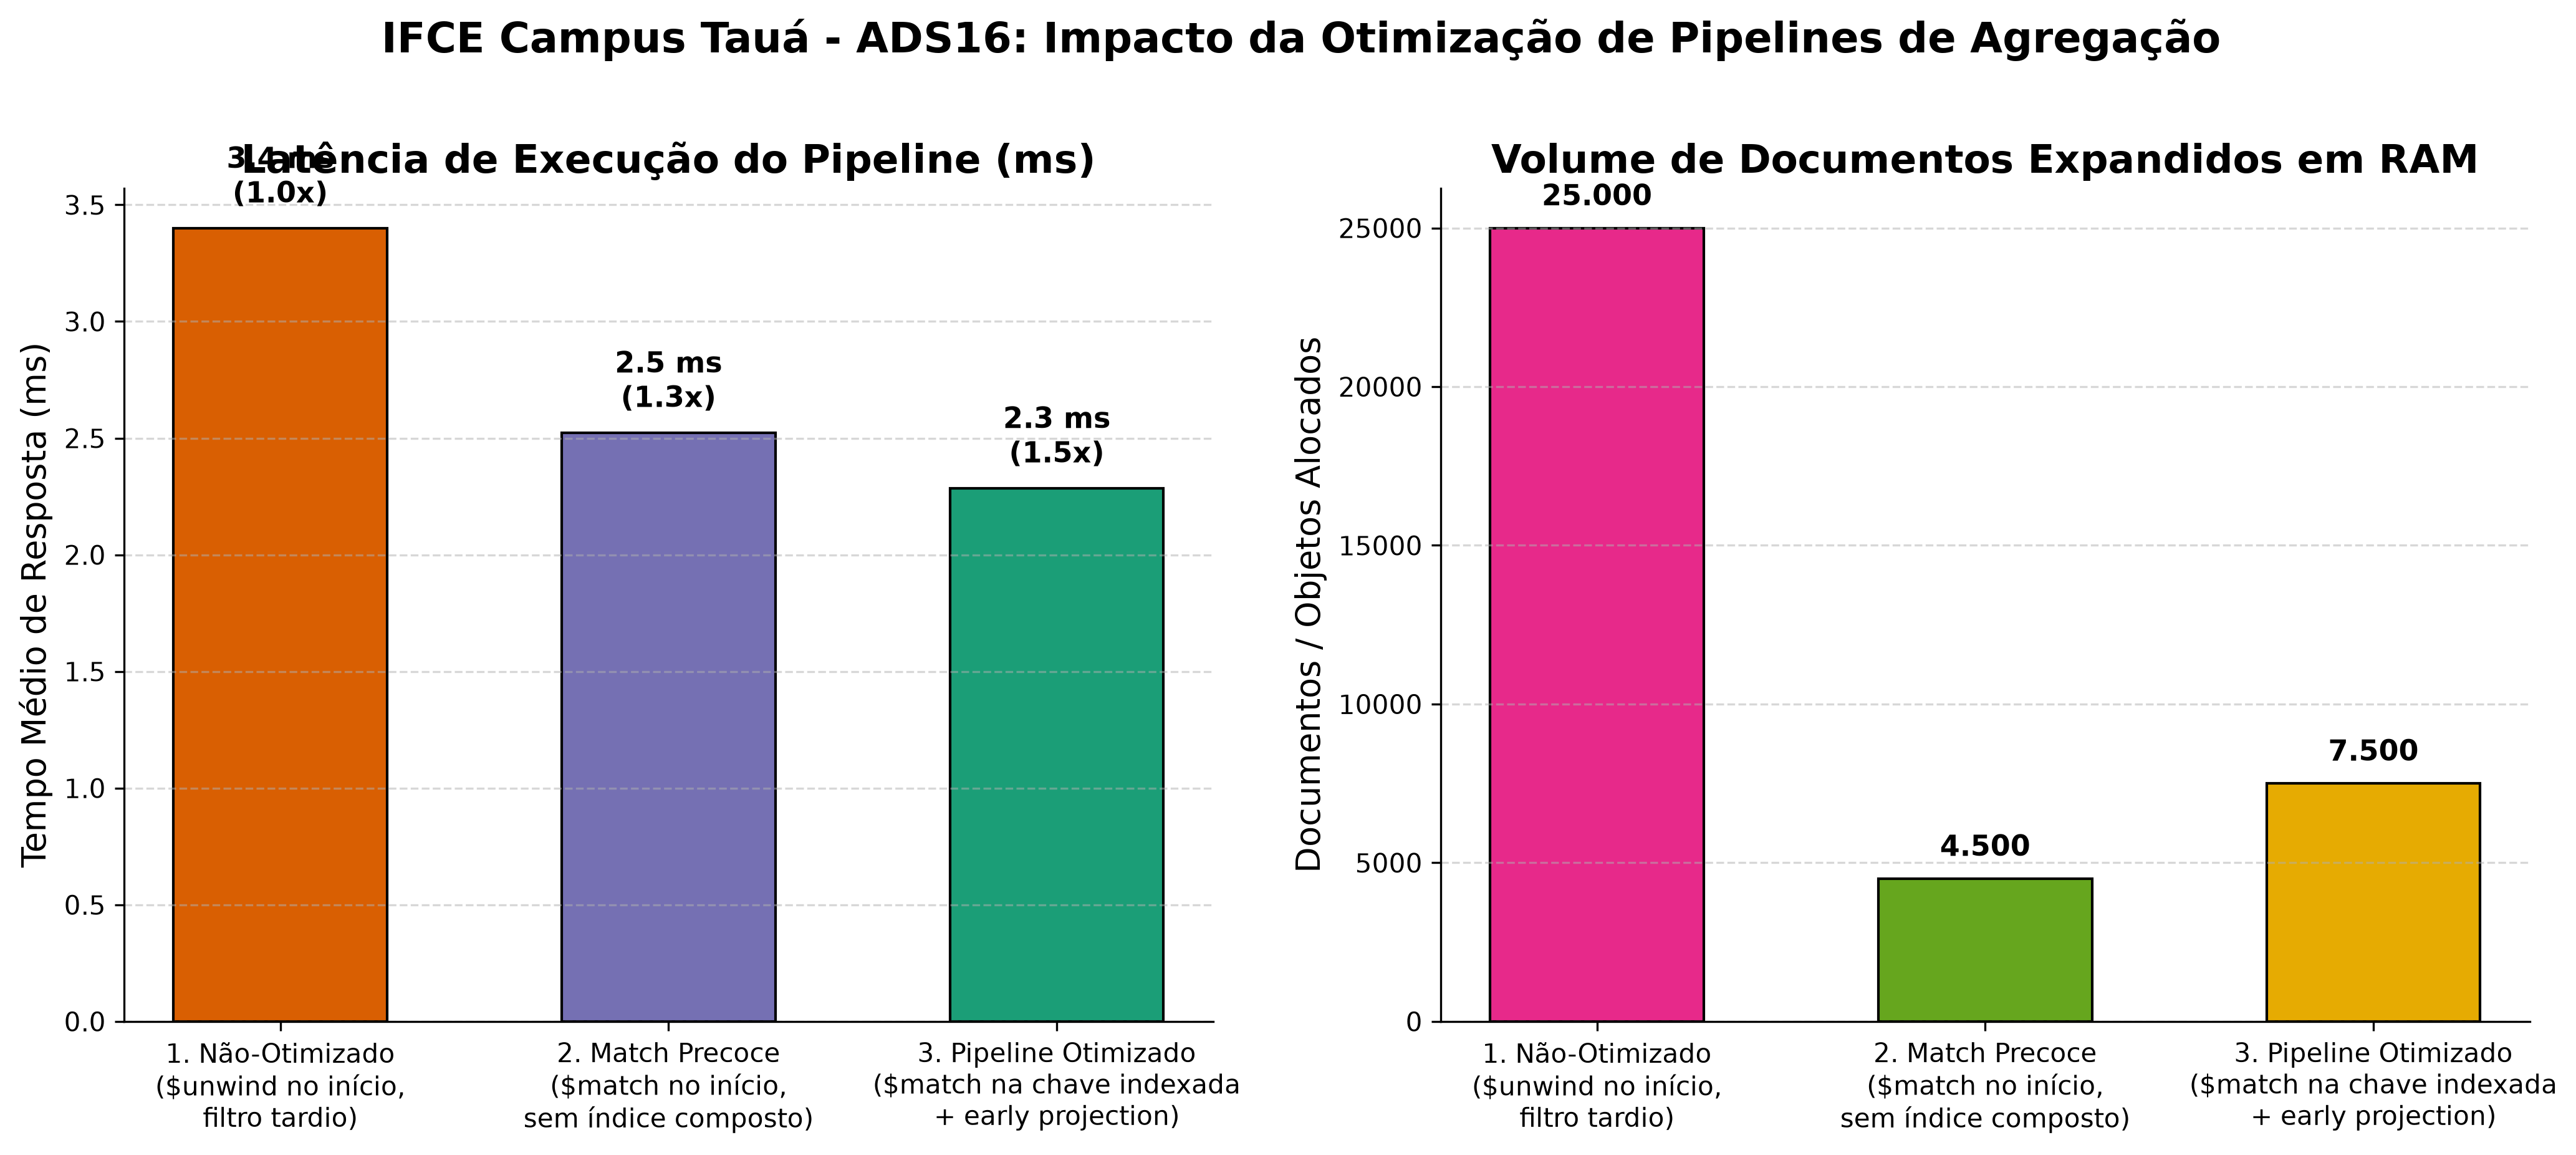
\includegraphics[width=\linewidth, height=4.2cm, keepaspectratio]{benchmark_aggregation_opt.png}
    \end{column}
  \end{columns}
\end{frame}
